\chapter{Graph models}
\label{chap:gnns}

\begin{supportbox}{About this chapter}
In this chapter we consider graph-structured data, i.e., nodes connected by a set of (known) relations. Graph are pervasive in the real world, ranging from proteins to traffic networks, social networks, and recommender systems. We introduce specialized layers to work on graphs, broadly categorized as either message-passing layers or graph transformers architectures.
\end{supportbox}

\section{Learning on graph-based data}
\subsection{Graphs and features on graphs}

Up to now we have considered data which is either completely unstructured  (tabular data represented as a vector) or structured in simple ways, including sets, sequences, and grids such as images. However, many types of data are defined by more sophisticated dependencies between its constituents. For example, molecules are composed by atoms which are only sparsely connected via chemical bonds. Networks of many kinds (social networks, transportation networks, energy networks) are composed of millions of units (people, products, users) which interact only through a small set of connections, e.g., roads, feedbacks, or friendships. These are more naturally defined in the language of \textbf{graph theory}. The aim of this chapter is to introduce differentiable models to work with data defined in such a way.

\begin{figure}[t]
    \centering
    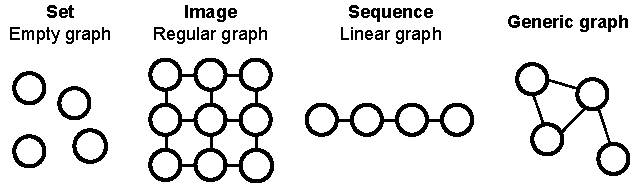
\includegraphics[width=0.8\textwidth]{images/graphs}
    \caption{Graphs generalize many types of data: sets can be seen as empty graphs (or graphs having only self-loops), images as regular graphs, and sequences as linear graphs. In this chapter we look at more general graph structures.}
    \label{fig:graphs}
\end{figure}

In its simplest form, a graph can be described by a pair of sets $\mathcal{G} = (\mathcal{V}, \mathcal{E})$, where $\mathcal{V} = \left\{1, \ldots, n\right\}$ is the set of \textbf{nodes} (\textbf{vertices}), while:
%
$$
\mathcal{E} = \left\{(i,j) \mid \eqnmarkbox[drawred]{node}{i,j \in \mathcal{N}}\right\}
$$
\annotate[yshift=-1em]{below,right}{node}{Two nodes of the graph}

is the set of \textbf{edges} present in the graph. In most datasets, the number of nodes $n$ and the number of edges $m = \lvert \mathcal{E}\rvert$ can vary from graph to graph. 

Graph generalize many concepts we have already seen: for example, graphs containing only \textbf{self-loops} of the form $(i,i)$ represent sets of objects, while graphs containing all possible edges (\textbf{fully-connected graphs}) are  connected to attention layers, as we show next. Images can be represented as a graph by associating each pixel to a node of the graph and connecting close pixels based on a regular grid-like structure - see Figure \ref{fig:graphs}.\footnote{There are many variants of this basic setup, including heterogenous graphs (graphs with different types of nodes), directed graphs, signed graphs, etc. Most of them can be handled by variations of the techniques we describe next.}

Connections in a graph can be equivalently represented by a matrix representation called the \textbf{adjacency matrix}. This is a binary square matrix $\mathbf{A} \sim \text{Binary}(n,n)$ such that:
%
$$
A_{ij} = \begin{cases} 1 & \text{ if } (i,j) \in \mathcal{E} \\ 0 & \text{ otherwise} \end{cases}
$$
%
In this format, a set is represented by the identity matrix $\mathbf{A} = \mathbf{I}$, a fully-connected graph by a matrix of all ones, and an image by a Toeplitz matrix. A graph where connections are always bidirectional (i.e., $(i,j)$ and $(j,i)$ are always present as pairs among the edges) is called \textbf{undirected}, and we have $\mathbf{A}^\top = \mathbf{A}$. We will deal with undirected graphs for simplicity, but the methods can be easily extended to the directed case. We note that there are also alternative matrix representations, e.g., the incidence matrix $\mathbf{B} \sim \text{Binary}(n, \lvert \mathcal{E}\rvert)$ is such that $B_{ij} = 1$ if node $i$ participates in edge $j$, and we have $\mathbf{B}\mathbf{1}^\top = 2$ because each edge connects exactly two nodes. See Figure \ref{fig:adjacency_matrix} for an example.

\begin{figure}[t]
    \centering
    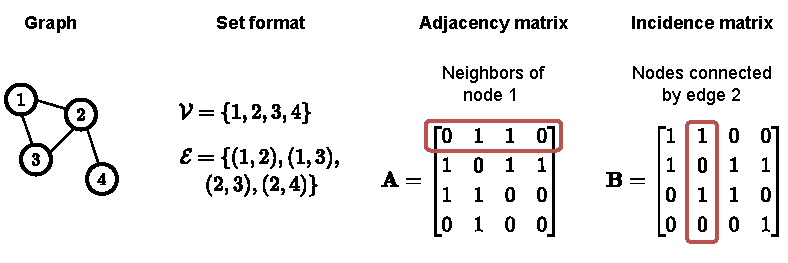
\includegraphics[width=1.0\textwidth]{images/graphs-2}
    \caption{We can represent the graph connectivity in three ways: as a set $\mathcal{E}$ of pairs (second column); as an $(n, n)$ adjacency matrix (third column); or as an $(n, \lvert \mathcal{E} \rvert)$ incidence matrix (fourth column).}
    \label{fig:adjacency_matrix}
\end{figure}

We will assume our graphs to have self-loops, i.e., $A_{ii} = 1$. If the adjacency matrix does not have self-loops, we can add them by re-assigning it as:
%
$$
\mathbf{A} \gets\mathbf{A} + \mathbf{I}
$$

\subsection{Graph features}

Graphs come with a variety of possible features describing them. For example, atoms and bonds in a molecule can be described by categorical features denoting their types; roads in a transportation network can have a capacity and a traffic flow; and two friends in a social networks can be described by how many years they have known each other.

In general, these features can be of three types: \textbf{node features} associated to each node, \textbf{edge features} associated to each edge, and \textbf{graph features} associated to the entire graph. We will begin with the simplest case of having access to only unstructured node features, i.e., each node $i$ has associated a vector $\mathbf{x}_i \sim (c)$. The complete graph can then be described by two matrices $\mathbf{X} \sim (n,c)$, that we call the \textbf{feature matrix}, and the adjacency matrix $\mathbf{A} \sim (n,n)$.

In most cases, the ordering of the nodes is irrelevant, i.e., if we consider a permutation matrix $\mathbf{P} \sim \text{Binary}(n,n)$ (see Section \ref{sec:positional_embeddings}), a graph and its permuted version are fundamentally identical, in other words:

$$
(\mathbf{X}, \mathbf{A}) \;\; \text{ is the same graph as } \;\;(\mathbf{P}\mathbf{X},\mathbf{P}\mathbf{A}\mathbf{P}^\top)
$$

Note that the permutation matrix acts by swapping the rows in $\mathbf{X}$, while it swaps both rows and columns in the adjacency matrix.

Some features can also be extracted directly from the topology of the graph. For example, we can associate to each node a scalar value $d_i$, called the \textbf{degree}, which describes how many nodes it is connected to:

$$
d_i=\sum_j A_{ij}
$$

The distribution of the degrees across the graph is an important characteristic of the graph itself, as shown in Figure \ref{fig:random_graphs}. We can collect the degrees into a single diagonal matrix called the \textbf{degree} matrix:

$$
\mathbf{D} =\begin{bmatrix} d_1 & \ldots & 0 \\ \vdots &\ddots & \vdots \\0 & \ldots & d_n \end{bmatrix}
$$

We can use the degree matrix to define several types of of \textit{weighted} adjacency matrices. For example, the row-normalized adjacency matrix is defined as:

$$
\mathbf{A}^\prime \leftarrow \mathbf{D}^{-1}\mathbf{A}_{ij} \;\; \rightarrow\;\; A^\prime_{ij} = \frac{1}{d_i}A_{ij}
$$



This is normalized in the sense that $\sum_i A^\prime_{ij} = \mathbf{1}$. We can also define a column-normalized adjacency matrix as $\mathbf{A}^\prime = \mathbf{A}\mathbf{D}^{-1}$. Both these matrices can be interpreted as “random walks” over the graph, in the sense that, given a node $i$, the corresponding row or column of the normalized adjacency matrix represents a probability distribution of moving at random towards any of its neighbours. A more general symmetrically normalized adjacency matrix is given by:

$$
\mathbf{A}^\prime=\mathbf{D}^{-1/2}\mathbf{A}\mathbf{D}^{-1/2}
$$

This is defined by $A^\prime_{ij} = \frac{A_{ij}}{\sqrt{d_i d_j}}$, giving a weight to each connection based on the degree of both nodes it connects to. Both the adjacency matrix and its weighted variants have the property that $A_{ij} = 0$ whenever $(i,j) \notin \mathcal{E}$. In signal processing terms, these are called \textbf{graph-shift} matrices.

\begin{supportbox}{Sparsity in matrices}
Consider a generic adjacency matrix for a $6$-nodes graph (try drawing the graph as an exercise):
%
$$
\mathbf{A} = \begin{bmatrix} 0& 1& 1& 1& 1& 1\\1& 0& 0& 0& 1& 0\\1& 0& 0& 0& 1& 1\\1& 0& 0& 0& 0& 1\\1& 1& 1& 0& 0& 0\\1& 0& 1& 1& 0& 0\end{bmatrix}
$$

The adjacency is very sparse (many zeros). This is an important property, because sparse matrices have customized implementations and techniques for manipulating them, with better computational complexity than their dense counterparts.\footnote{As an example, in JAX: \url{https://jax.readthedocs.io/en/latest/jax.experimental.sparse.html}.}
\end{supportbox}

\begin{figure}[t]
    \centering
    \begin{subfigure}[b]{0.24\textwidth}
    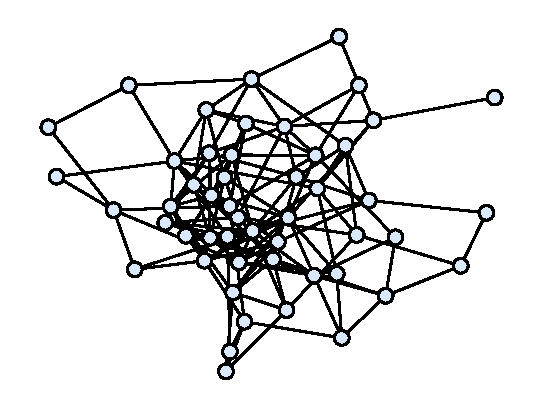
\includegraphics[width=\textwidth]{images/graph_1}
    \caption{Erdős–Rényi}
    \end{subfigure}
    \begin{subfigure}[b]{0.24\textwidth}
    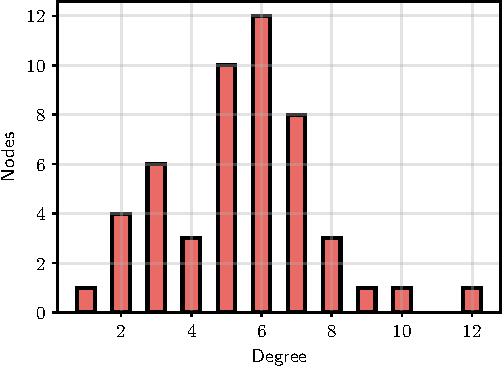
\includegraphics[width=\textwidth]{images/graph_1_degree}
    \caption{Degree}
    \end{subfigure}
    \begin{subfigure}[b]{0.24\textwidth}
    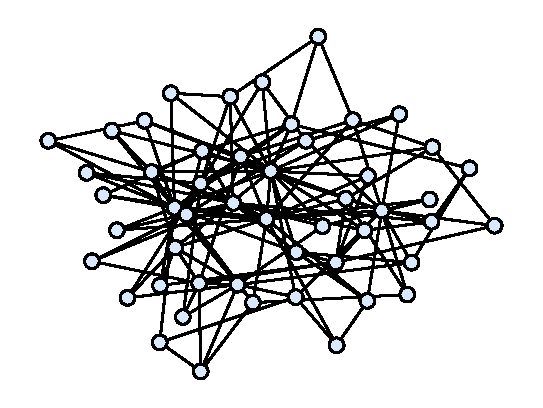
\includegraphics[width=\textwidth]{images/graph_2}
    \caption{Barabasi-Albert}
    \end{subfigure}
    \begin{subfigure}[b]{0.24\textwidth}
    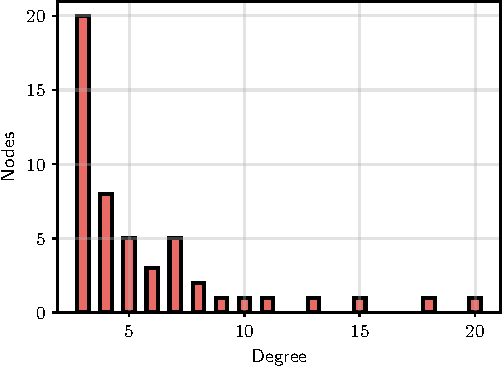
\includegraphics[width=\textwidth]{images/graph_2_degree}
    \caption{Degree}
    \end{subfigure}
    \caption{(a) Random graph generated by drawing each edge independently from a Bernoulli distribution (\textbf{Erdős–Rényi model}). (b) These graphs show a Gaussian-like degree distribution. (c) Random graph generated by adding nodes sequentially, and for each of them drawing $3$ connections towards existing nodes with a probability proportional to their degree (\textbf{preferential attachment process} or \textbf{Barabasi-Albert model}). (d) These graphs have a few nodes with many connections acting as hubs for the graph.}
    \label{fig:random_graphs}
\end{figure}

\subsection{Diffusion operations over graphs}

The fundamental graph operation we are interested into is something called \textbf{diffusion}, which corresponds to a smoothing of the node features with respect to the graph topology. To understand it, consider a scalar feature on each node, that we collect in a vector $\mathbf{x} \sim (n)$, and the following operation over the features:

$$
\mathbf{x}^\prime=\mathbf{A}\mathbf{x}
$$

where $\mathbf{A}$ can be the adjacency matrix, a normalized variant, or any weighted adjacency matrix. We can re-write this operation node-wise as:

$$
x^\prime_i = \sum_{j \in \mathcal{N}(i)} A_{ij}x_j
$$

where we have defined the $1$-hop neighborhood:

\vspace{1em}
$$
\mathcal{N}(i) = \left\{ j\mid \eqnmarkbox[drawred]{node}{(i,j)\in\mathcal{E}} \right\}
$$
\annotate[yshift=1em]{above,right}{node}{All edges with node $i$ as a vertex}

\vspace{-1em}
If we interpret the node feature as a physical quantity, projection by the adjacency matrix can be seen as a “diffusion” process which replaces the quantity at each node by a weighted average of the quantity in its neighborhood.

Another fundamental matrix in the context of graph analysis is the \textbf{Laplacian matrix}:

$$
\mathbf{L}=\mathbf{D}-\mathbf{A}
$$

where the degree matrix is computed as $D_{ii} = \sum_j A_{ij}$ irrespective of whether the adjacency matrix is normalized or not. One step of diffusion by the Laplacian can be written as:

\begin{equation}
\mathbf{L}\mathbf{x}=\sum_{(i,j) \in \mathcal{E}} A_{ij}(x_i-x_j)
\label{eq:laplacian}
\end{equation}

\begin{figure}[t]
    \centering
    \begin{subfigure}[b]{0.24\textwidth}
    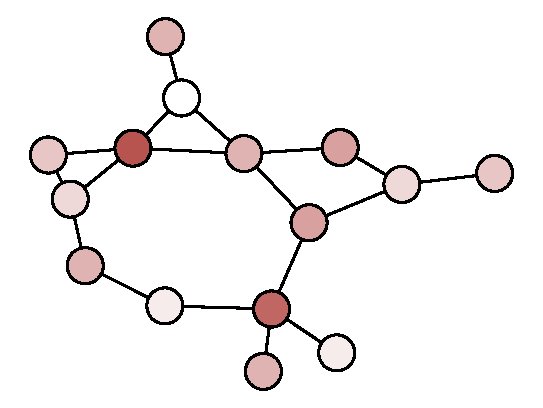
\includegraphics[width=\textwidth]{images/graph_diffusion_0}
    \caption{Initial graph}
    \end{subfigure}
    \begin{subfigure}[b]{0.24\textwidth}
    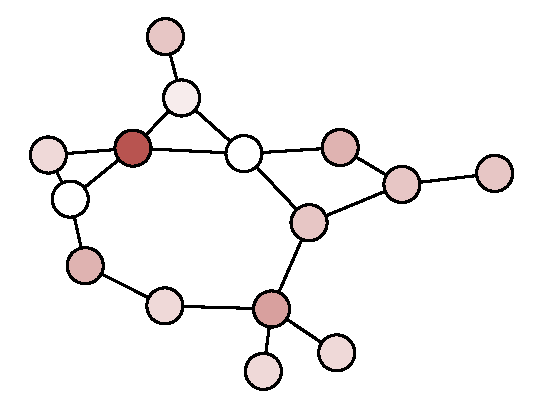
\includegraphics[width=\textwidth]{images/graph_diffusion_10}
    \caption{10 steps}
    \end{subfigure}
    \begin{subfigure}[b]{0.24\textwidth}
    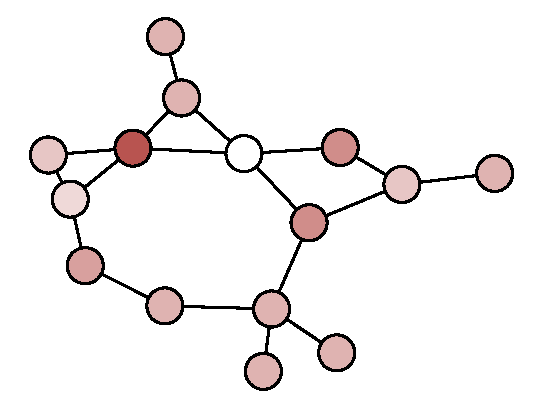
\includegraphics[width=\textwidth]{images/graph_diffusion_20}
    \caption{20 steps}
    \end{subfigure}
    \begin{subfigure}[b]{0.24\textwidth}
    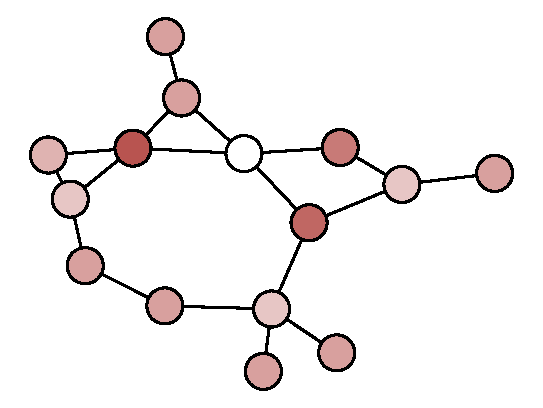
\includegraphics[width=\textwidth]{images/graph_diffusion_30}
    \caption{30 steps}
    \end{subfigure}
    \caption{(a) A random graph with 15 nodes and a scalar feature on each node (denoted with variable colors). (b)-(d) The result after $10$, $20$, and $30$ steps of diffusion with the Laplacian matrix. The features converge to a stable state.}
    \label{fig:diffusion}
\end{figure}

We can see from here that the Laplacian is intimately linked to the idea of a gradient over a graph, and its analysis is at the core of the field of \textbf{spectral graph theory}. As an example, in \eqref{eq:laplacian} $\mathbf{1}$ is always an eigenvector of the Laplacian associated to a zero eigenvalue (in particular, the smallest one). We show an example of diffusion with the Laplacian matrix in Figure \ref{fig:diffusion}.



\subsection{Manifold regularization}

From \eqref{eq:laplacian} we can also derive a quadratic form built on the Laplacian:

\begin{equation}
\mathbf{x}^\top\mathbf{L}\mathbf{x}=\sum_{(i,j)\in \mathcal{E}}A_{ij}(x_i-x_j)^2
\label{eq:laplacian_regularizer}
\end{equation}

Informally, this is a scalar value that measures how “smooth” the signal over the graph is, i.e., how quickly it changes for pairs of nodes that are connected in the graph. To see a simple application of this concept, consider a tabular classification dataset $\mathcal{S}_n = \left\{(\mathbf{x}_i, y_i)\right\}$. Suppose we build a graph over this dataset, where each node is an element of the dataset, and the adjacency matrix is built based on the distance between features:

\begin{equation}
A_{ij}=\begin{cases} \exp(-\lVert \mathbf{x}_i - \mathbf{x}_j \rVert^2) & \text{ if } \lVert \mathbf{x}_i - \mathbf{x}_j \rVert^2 < \tau \\ 0 & \text{otherwise} \end{cases}
\label{eq:dataset_graph}
\end{equation}

where $\tau$ is a user-defined hyper-parameter. Given a classification model $f(\mathbf{x})$, we may want to constrain its output to be similar for similar inputs, where similarity is defined proportionally to \eqref{eq:dataset_graph}. To this end, we can define the features of the graph as the outputs of out model:

$$
\mathbf{f} = \begin{bmatrix} f(\mathbf{x}_1) \\ \vdots \\ f(\mathbf{x}_n) \end{bmatrix} \sim (n)
$$

The quadratic form \eqref{eq:laplacian_regularizer} tells us exactly how much similar inputs vary in terms of their predictions:

\begin{equation}
\mathbf{f}^\top\mathbf{L}\mathbf{f} = \sum_{i,j} A_{ij}(f(\mathbf{x}_i)-f(\mathbf{x}_j))^2
\label{eq:manifold_regularizer}
\end{equation}

The optimal model can be found by a regularized optimization problem, where the regularizer is given by \eqref{eq:manifold_regularizer} :
%
$$
f^*(\mathbf{x})=\arg\min \left\{\sum_{i=1}^nL(y_i, f(\mathbf{x}))  + \lambda \;\;\mathbf{f}^\top \mathbf{L}\mathbf{f}\right\}
$$
%
where $L$ is a generic loss function and $\lambda$ is a scalar hyper-parameter:

This is called \textbf{manifold regularization} \cite{belkin2006manifold} and it can be used as a generic regularization tool to force the model to be smooth over a graph, where the adjacency is either given or is built by the user as in \eqref{eq:dataset_graph}. This is especially helpful in a \textbf{semi-supervised} scenario where we have a small labeled dataset and a large unlabeled one from the same distribution, since the regularizer in \eqref{eq:manifold_regularizer} does not require labels \cite{belkin2006manifold}. However, the prediction of the model depends only on a single element $\mathbf{x}_i$, and the graph is thrown away after training. In the next section, we will introduce more natural ways of embedding the connectivity inside the model itself.

\section{Graph convolutional layers}
\subsection{Properties of a graph layer}

In order to design models whose predictions are conditional on the connectivity, we can augment standard layers $f(\mathbf{X})$ with knowledge of the adjacency matrix, i.e., we consider layers of the form:
%
$$
\mathbf{H} =f(\mathbf{X}, \mathbf{A})
$$
%
where as before $\mathbf{X} \sim (n, c)$ (with $n$ the number of nodes and $c$ the features at each node) and $\mathbf{H} \sim (n, c^\prime)$, i.e., the operation does not change the connectivity of the graph, and it returns an updated embedding $\mathbf{H}_i \sim (c^\prime)$ for each node $i$ in the graph. For what follows, $\mathbf{A}$ can be the adjacency or any matrix with the same sparsity pattern (a graph-shift matrix), including a weighted adjacency matrix, the Laplacian matrix, and so on.

Since permuting the nodes in a graph should have no impact on the final predictions, the layer should not depend on the specific ordering of the nodes, i.e., for any permutation matrix $\mathbf{P}$ the output of the layer should be \textbf{permutation equivariant}:
%
$$
f(\mathbf{P}\mathbf{X}, \mathbf{P}\mathbf{A}\mathbf{P}^\top)=\mathbf{P}\,\cdot\,f(\mathbf{X}, \mathbf{A})
$$
%
We can define a notion of “locality” for a graph layer, similar to the image case. To this end, we first introduce the concept of a subgraph. Given a subset of nodes $\mathcal{T} \in \mathcal{V}$ from the full graph, we define the \textbf{subgraph} induced by $\mathcal{T}$ as:
%
$$
\mathcal{G}_{\mathcal{T}}= (\mathbf{X}_{\mathcal{T}}, \mathbf{A}_{\mathcal{T}})
$$
%
where $\mathbf{X}_{\mathcal{T}}$ is a $(\lvert\mathcal{T}\rvert,c)$ matrix collecting the features of the nodes in $\mathcal{T}$, and $\mathbf{A} \sim (\lvert\mathcal{T}\rvert,\lvert\mathcal{T}\rvert)$ is the corresponding block of the full adjacency matrix.

\begin{definition}[Graph locality]
A graph layer $\mathbf{H} =f(\mathbf{X}, \mathbf{A})$ is \textbf{local} if for every node, $\mathbf{H}_i = f(\mathbf{X}_{\mathcal{N}(i)}, \mathbf{A}_{\mathcal{N}(i)})$, where $\mathcal{N}(i)$ is the $1$-hop neighborhood of node $i$.
\end{definition}

This is similar to considering all pixels at distance $1$ in the image case, except that (a) nodes in $\mathcal{N}(i)$ have no specific ordering in this case, and (b) the size of $\mathcal{N}(i)$ can vary a lot depending on $i$. Hence, we cannot define a convolution like we did in the image case, as its definition requires these two properties (think of the weight tensor in a convolutional layer).

For what follows, note that we can extend our definition of locality beyond 1-hop neighbors. For example, the 2-hop neighborhood $\mathcal{N}^2(i)$ is defined as all nodes at distance at most $2$:
%
$$
\mathcal{N}^2(i) = \bigcup_{j \in \mathcal{N}(i)} \mathcal{N}(j) 
$$
%
where $\cup$ is the set union operator. We can extend the definition of locality to take higher-order neighborhoods into consideration and design the equivalent of $3 \times 3$ filters, $5 \times 5$ filters, and so on.

\subsection{The graph convolutional layer} \addclock

In order to define a graph layer that mimicks the convolutional layer, we need it to be permutation equivariant (instead of translation equivariant) and local. The MHA layer is naturally permutation equivariant, but it is not local and it does not depend explicitly on the adjacency matrix $\mathbf{A}$. We will see possible extensions to this end in the next section. For now, let us focus on a simpler fully-connected layer:
%
$$
f(\mathbf{X}, \_)= \phi(\mathbf{X}\mathbf{W}+\mathbf{b})
$$
%
where $\mathbf{W} \sim (c^\prime,c)$ and $\mathbf{b} \sim (c^\prime)$. This is also naturally permutation equivariant, but it does not depend on the connectivity of the graph, which is ignored. To build an appropriate differentiable layer, we can alternate the layer's operation with a diffusion step.

\begin{definition}[Graph convolution] \addbottle
%
Given a graph represented by a node feature matrix $\mathbf{X} \sim (n,c)$ and a generic graph-shift matrix $\mathbf{A} \sim (n,n)$ (the adjacency, the Laplacian, ...), a \textbf{graph convolutional} (GC) layer is given by \cite{kipf2016semi}:
%
$$
f(\mathbf{X}, {\color{drawred}\mathbf{A}})= \phi({\color{drawred}\mathbf{A}}(\mathbf{X}\mathbf{W}+\mathbf{b}))
$$
%
where the trainable parameters are $\mathbf{W} \sim (c^\prime,c)$ and $\mathbf{b} \sim (c^\prime)$, with $c^\prime$ an hyper-parameter. $\phi$ is a standard activation function, such as a ReLU.
\end{definition}

\begin{SCfigure}
    \centering
    \hspace{2em}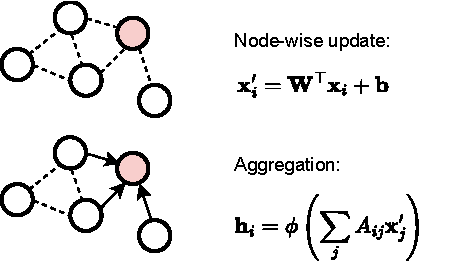
\includegraphics[width=0.5\textwidth]{images/graph_convolution_layer}
    \caption{Two stages of a GC layer: each node updates its embedding in parallel to all other nodes; the output is given by a weighted average of all updated embeddings in the node's neighbourhood.}
    \label{fig:graph_convolution_layer}
\end{SCfigure}

Note the similarity with a standard convolutional layer: we are performing a “channel mixing” operation via the matrix $\mathbf{W}$, and a “node mixing” operation via the matrix $\mathbf{A}$, the difference being that the former is untrainable in this case (due to, once again, variable degrees between nodes and the need to make the layer permutation equivariant). See Figure \ref{fig:graph_convolution_layer} for a visualization. The analogy can also be justified more formally by leveraging concepts from graph signal processing, which is beyond the scope of this book \cite{bronstein2017geometric}. Ignoring the bias, we can rewrite this for a single node $i$ as:

$$
\mathbf{H}_i=\phi\left(\sum_{j \in \mathcal{N}(i)}A_{ij}\mathbf{X}_j\mathbf{W}\right)
$$

Hence, we first perform a simultaneous update of all node embeddings (given by the right multiplication by $\mathbf{W}$). Then, each node computes a weighted average of the updated node embeddings from itself and its neighbors. Since the number of neighbors can vary from node to node, working with the normalized variants of the adjacency matrix can help significantly in training. It is trivial to show permutation equivariance for the layer:

$$
f({\color{drawred}\mathbf{P}}\mathbf{X},{\color{drawred}\mathbf{P}}\mathbf{A}{\color{drawred}\mathbf{P}^\top})=\phi\left({\color{drawred}\mathbf{P}}\mathbf{A}{\color{drawred}\mathbf{P}^\top}{\color{drawred}\mathbf{P}}\mathbf{X}\mathbf{W}\right) = {\color{drawred}\mathbf{P}}\,\cdot\,f(\mathbf{X},\mathbf{A})
$$

\subsection{Building a graph convolutional network}

A single GC layer is local, but the stack of multiple layers is not. For example, consider a two-layered GC model:

\begin{equation}
f(\mathbf{X},\mathbf{A})=\phi(\mathbf{A}\eqnmarkbox[drawred]{node}{\phi\left(\mathbf{A}\mathbf{X}\mathbf{W}_1\right)}\mathbf{W}_2)
\label{eq:two_layer_gcn}
\end{equation}
\annotate[yshift=-1em]{below,right}{node}{First GC layer}

\vspace{1em}
with two trainable weight matrices $\mathbf{W}_1$ and $\mathbf{W}_2$. Similarly to the image case, we can define a notion of receptive field.

\begin{definition}[Graph receptive field]
Given a generic graph neural network $\mathbf{H} = f(\mathbf{X}, \mathbf{A})$, the \textbf{receptive field} of node $i$ is the smallest set of nodes $\mathcal{V}(i) \in \mathcal{V}$ such that $\mathbf{H}_i = f(\mathbf{X}_{\mathcal{V}(i)}, \mathbf{A}_{\mathcal{V}(i)})$.
\end{definition}

For a single GC layer, the receptive field is $\mathcal{V}(i) = \mathcal{N}(i)$. For a two-layer network as in  \eqref{eq:two_layer_gcn}, we need to consider neighbors of neighbors, and the receptive field becomes $\mathcal{V}(i) = \mathcal{N}^2(i)$. In general, for a stack of $k$ layers we will have a receptive field of $\mathcal{V}(i) = \mathcal{N}^k(i)$. The smallest number of steps which is needed to move from any two nodes in the graph is called the \textbf{diameter} of the graph. The diameter defines the smallest number of layers which is required to achieve a global receptive field for all the nodes. 

\begin{supportbox}{Polynomial GC layers}

Alternatively, we can increase the receptive field of \textit{a single} GC layer. For example, if we remove the self-loops from the adjacency matrix, we can make the layer local with respect to $\mathcal{N}^2(i)$ instead of $\mathcal{N}(i)$ by also considering the square of the adjacency matrix:

$$
\mathbf{H} = \phi\left(\mathbf{X}\mathbf{W}_0 + \mathbf{A}\mathbf{X}\mathbf{W}_1 + \mathbf{A}^2\mathbf{X}\mathbf{W}_2\right)
$$

where we have three sets of parameters $\mathbf{W}_0$, $\mathbf{W}_1$, and $\mathbf{W}_2$ to handle self-loops, neighbors, and neighbors of neighbors respectively. This is called a \textbf{polynomial} GC layer. Larger receptive fields can be obtained with higher powers. More complex layers can be designed by considering ratios of polynomials \cite{bianchi2021graph}.

\end{supportbox}

We can combine GC layers with standard normalization layers, residual connections, dropout, or any other operation that is permutation equivariant. Differently from the image case, pooling is harder because there is no immediate way to subsample a graph connectivity. Pooling layers can still be defined by leveraging tools from graph theory or adding additional trainable components, but they are less common \cite{grattarola2022understanding}.

Denote by $\mathbf{H} = f(\mathbf{X}, \mathbf{A})$ a generic combination of layers providing an updated embedding for each node (without modifying the connectivity). In analogy with CNNs, we call it the \textbf{backbone} network. We can complete the design of a generic \textbf{graph convolutional network} (GCN) by adding a small head of top of these representations:
%
$$
y=(g\circ f)(\mathbf{X},\mathbf{A})
$$
%
The design of the head depends on the task we are trying to solve. The most common tasks fall into one of three basic categories: node-level tasks (e.g., node classification), edge-level task (e.g., edge classification), or graph-level tasks (e.g., graph classification). We briefly consider an example for each of them in turn, see Figure \ref{fig:graph_heads}.

\begin{figure}[t]
    \centering
    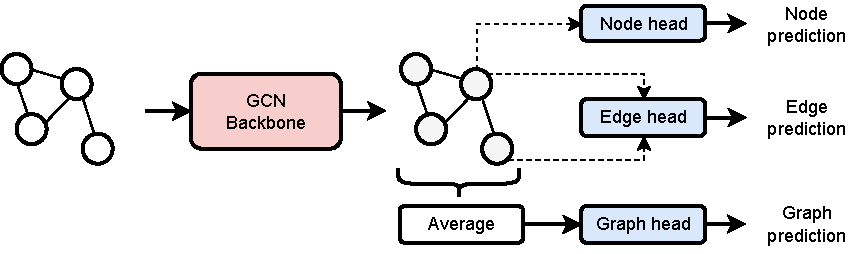
\includegraphics[width=0.9\textwidth]{images/graph_heads}
    \caption{Different types of graph heads: (a) node tasks need to process the features of a single node; (b) edge tasks require heads that are conditioned on two nodes simultaneously; (c) graph tasks can be achieved by pooling all node representations into a fixed-dimensional vector.}
    \label{fig:graph_heads}
\end{figure}

\textbf{Node classification}

First, suppose the input graph describes some kind of social network, where each user is associated to a node. For a given subset of users, $\mathcal{T} \subseteq \mathcal{V}$, we know a label $y_i, i \in \mathcal{T}$ (e.g., whether the user if a real user, a bot, or another kind of automated profile). We are interested in predicting the label for all other nodes. In this case, we can obtain a node-wise prediction by processing each updated node embedding, e.g.:

$$
\hat{y}_i=g(\mathbf{H}_i) =\text{softmax}(\text{MLP}(\mathbf{H}_i))
$$

Running this operation over the entire matrix $\mathbf{H}$ gives us a prediction for all nodes, but we only know the true labels for a small subset. We can train the GCN by discarding the nodes outside of the training set:

$$
\arg\min \frac{1}{\lvert \mathcal{T} \rvert}\sum_{i \in \mathcal{T}} \text{CE}(\hat{y}_i,y_i)
$$

where $\text{CE}$ is the cross-entropy loss. Importantly, even if we are discarding the output predictions for nodes outside our training set, their input features are still involved in the training process due to the diffusion steps inside the GCN. The rest of the nodes can then be classified by running the GCN a final time after training. This scenario, where only a subset of the training data is labeled, is called a \textbf{semi-supervised} problem.

\textbf{Edge classification}

As a second example, suppose we have a label for a subset of \textit{edges}, i.e., $\mathcal{T}_E \subseteq \mathcal{E}$. As an example, our graph could be a traffic network, of which we know the traffic flow only on a subset of roads. In this case, we can obtain an edge-wise prediction by adding an head that depends on the features of the two connected nodes, e.g., by concatenating them:

$$
\hat{y}_{ij} = g(\mathbf{H}_i, \mathbf{H}_j)= \text{MLP}\left(\left[ \mathbf{H}_i \;\Vert \; \mathbf{H}_j\right]\right)
$$

For binary classification (e.g., predicting the affinity of two users with a scalar value between $0$ and $1$) we can simplify this by considering the dot product between the two features:

$$
\hat{y}_{ij} = \sigma( \mathbf{H}_i^\top \mathbf{H}_j)
$$

Like before, we can train the network by minimizing a loss over the known edges.

\textbf{Graph classification}

Finally, suppose we are interested in classifying (or regressing) the entire graph. As an example, the graph could be a molecule of which we want to predict some chemical property, such as reactivity against a given compound. We can achieve this by pooling the node representations (e.g., via a sum), and processing the resulting fixed-dimensional embedding:

$$
y=\text{MLP}\left(\frac{1}{n}\sum_{i=1}^n \mathbf{H}_i\right)
$$

The final pooling layer makes the network \textit{invariant} to the permutation of the nodes. In this case, our dataset will be composed of multiple graphs (e.g., several molecules), making it similar to a standard image classification task. For node and edge tasks, instead, some datasets may be composed of a single graph (e.g., a large social network), while other datasets can have more than a single graph (e.g., several unconnected road networks from different towns). This opens up the question of how to efficiently build mini-batches of graphs.

\subsection{On the implementation of graph neural networks} \addteacup

As we mentioned, the peculiarity of working with graphs is that several matrices involved in our computations can be very sparse. For example, consider the following adjacency matrix:

$$
\mathbf{A} = \begin{bmatrix} 0 & 0 & 1 \\ 0 & 0 & 0 \\ 1 & 0 & 0 \end{bmatrix}
$$

This corresponds to a three-node graph with a single bidirectional edge between nodes $1$ and $3$. We can store this more efficiently by only storing the indices of the non-zero values, e.g., in code:

{\begin{center}\footnotesize
\noindent\mintinline{python}{A = [[0,2], [2,0]]}
\end{center}
}

This is called a \textbf{coordinate list} format. For very sparse matrices, specialized formats like this one can reduce storage but also significantly improve the runtime of operating on sparse matrices or on combinations of sparse and dense matrices. As an example, pytorch-sparse\footnote{\url{https://github.com/rusty1s/pytorch_sparse}} supports highly-efficient implementations of transposition and several types of matrix multiplications in PyTorch. This is also reflected on the layers’ implementation. The forward pass of the layers in PyTorch Geometric\footnote{\url{https://pytorch-geometric.readthedocs.io/en/latest/get_started/introduction.html\#learning-methods-on-graphs}} (one of the most common libraries for working with graph neural networks in PyTorch) is parameterized by providing as inputs the features of the graph and the connectivity as a list of edge coordinates.

\begin{SCfigure}
    \centering
    \hspace{2em}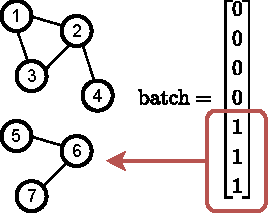
\includegraphics[width=0.4\textwidth]{images/graphs-Page-4}
    \caption{Two graphs in a mini-batch can be seen as a single graph with two disconnected components. In order to distinguish them, we need to introduce an additional vector containing the mapping between nodes and graph IDs.}
    \label{fig:graph_batch}
\end{SCfigure}

Working with sparse matrices has another interesting consequence in terms of mini-batches. Suppose we have $b$ graphs $(\mathbf{X}_i, \mathbf{A}_i)_{i=1}^b$. For each graph we have the same number of node features $c$ but a different number of nodes $n_i$, so that $\mathbf{X}_i \sim (n_i, c)$ and $\mathbf{A}_i \sim \text{Binary}(n_i, n_i)$. In order to build a mini-batch, we can create two rank-$3$ tensors:
%
\begin{gather}
X \sim (b,n,c) \\A\sim \text{Binary}(b,n,n)
\end{gather}
%
where $n = \max(n_1, \ldots, n_b)$, and both matrices are padded with zeros to fill up the two tensors. However, a more elegant alternative can be obtained by noting that in a GC layer, two nodes that are not connected by any path (a sequence of edges) will never communicate. Hence, we can build a \textit{single} graph describing the entire mini-batch by simply merging all the nodes:
%
\begin{gather}
\mathbf{X} = \begin{bmatrix}\mathbf{X}_1 \\ \vdots \\ \mathbf{X}_b \end{bmatrix} \\ \mathbf{A} = \begin{bmatrix} \mathbf{A}_1 & \ldots & \mathbf{0} \\ \vdots& \ddots & \vdots \\ \mathbf{0} & \ldots & \mathbf{A}_b \end{bmatrix}
\end{gather}
%
where $\mathbf{X} \sim (\sum_i n_i, c)$ and $\mathbf{A} \sim \text{Binary}(\sum_i n_i, \sum_i n_i)$. The adjacency matrix of the mini-batch has a block-diagonal structure, where all elements outside the diagonal blocks are zero (nodes from different graphs are not connected). While seemingly wasteful, this actually increases the sparsity ratio of the graph, making better use of the sparse matrix operations. Hence, for graph datasets in many cases there is no real difference between working with a single graph or a mini-batch of graphs.

In order to keep track which node belongs to each input graph, we can augment the representation with an additional vector $\mathbf{b} \sim (\sum_i n_i)$ such that $b_i$ is an index in $[1, \ldots, b]$ identifying one of the $b$ input graphs - see Figure \ref{fig:graph_batch}. For graph classification, we can exploit $\mathbf{b}$ to perform pooling separately on groups of nodes corresponding to different graphs. Suppose $\mathbf{H} \sim (n,c^\prime)$ is the output of the GCN backbone, then:
%
\begin{equation}
\text{scatter\_sum}\left(\mathbf{H}, \mathbf{b}\right) = \mathbf{Y} \sim (b, c^\prime)
\label{eq:scatter_sum}
\end{equation}
%
is called a \textbf{scattered sum} operation and is such that the $\mathbf{Y}_i$ is the sum of all rows of $\mathbf{H}$ such that $b_j = i$, as shown in Figure \ref{fig:scatter_sum}. Similar operations can be defined for other types of pooling operations, such as averages and maximums.

\begin{figure}[t]
    \centering
    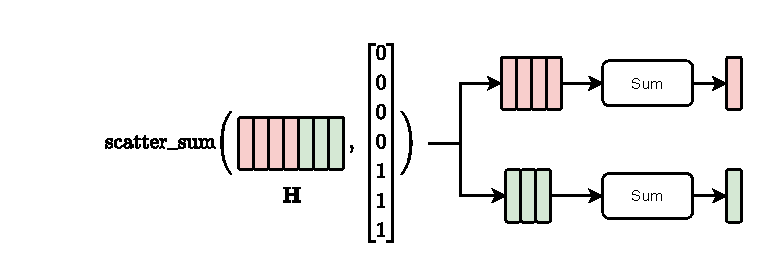
\includegraphics[width=0.9\textwidth]{images/graphs-Pagina-5}\hspace*{5em}
    \caption{Example of scattered sum on the graph of Figure \ref{fig:graph_batch}. In this example nodes (1,2,3,4) belong to graph 1, and nodes (5,6,7) to graph 2. After pooling, we obtain a pooled representation for each of the two graphs.}
    \label{fig:scatter_sum}
\end{figure}

As a separate problem, sometimes we may have a single graph that does not fit into memory: in this case, mini-batches should be formed by \textit{sampling} subgraphs from the original graph \cite{hamilton2017inductive}. This is a relatively complex task that goes beyond the scope of this chapter.

\section{Beyond graph convolutional layers}

With the GC layer as template, we now overview a few extensions, either in terms of adaptivity or graph features that can be handled. We close by discussing \textbf{graph transformers}, a different family of layers in which the graph is embedded into a structural embedding which is summed to the node features.

\subsection{Graph attention layers}

One issue with GC layers is that the weights that are used to sum up contributions from the neighborhoods are fixed and are given by the adjacency matrix (or a proper normalized variant). Most of the time this is equivalent to assuming that, apart from the relative number of connections, all neighbors are equally important. A graph where nodes are connected mostly with similar nodes is called \textbf{homophilic}: empirically, homophily is a good predictor of the performance of graph convolutional layers \cite{li2022graph}. Not all graphs are homophilic: for example, in a dating network, most people will be connected with people from the opposite sex. Hence, in these scenarios we need techniques that can properly adapt the weights given from each node to another node adaptively.

For sufficiently small graphs, we can let the non-zero elements of the weight matrix $\mathbf{A}$ adapt from their starting value through gradient descent. However, the number of trainable parameters in this case increases quadratically with the number of nodes, and this solution does not apply to a scenario with more than a single graph. If we assume that an edge depends only on the features of the two nodes it connects, we can generalize the GC layer with an attention-like operator:
%
$$
\mathbf{h}_i=\phi\left(\sum_{j \in \mathcal{N}(i)}{\color{drawred}\text{softmax}(\alpha(\mathbf{x}_i, \mathbf{x}_j))}\mathbf{W}^\top\mathbf{x}_j\right)
$$
%
where $\alpha$ is some generic MLP block having two inputs and a scalar output, and the softmax is applied, for each node, to the set of outputs of $\alpha$ with respect to $\mathcal{N}(i)$, to normalize the weights irrespective of the size of the neighborhood. Due to the similarity to the attention layer, these are called \textbf{graph attention} (GAT) layers \cite{velivckovic2017graph}. Seen from the perspective of the entire graph, this is very similar to a MHA layer, where the attention operation is restricted only on nodes having an edge that connects them.

The choice of $\alpha$ is relatively free. Instead of a dot product, the original GAT formulation considered an MLP applied on a concatenation of features:
%
$$
\alpha(\mathbf{x}_i, \mathbf{x}_j)=\text{LeakyReLU}(\mathbf{a}^\top \left[ \mathbf{V}\mathbf{x}_i \;\lVert\; \mathbf{V}\mathbf{x}_j \right])
$$
%
where $\mathbf{V}$ and $\mathbf{a}$ are trainable. This was later found to be restrictive, in the sense that the ordering between elements does not depend on the central node \cite{brody2021attentive}. A less restrictive variant, called \textbf{GATv2} \cite{brody2021attentive} is obtained as:
%
$$
\alpha(\mathbf{x}_i, \mathbf{x}_j)= \mathbf{a}^\top\text{LeakyReLU}( \mathbf{V}\left[ \mathbf{x}_i \;\lVert\; \mathbf{x}_j \right])
$$
%
Both GAT and GATv2 are very popular baselines nowadays.

\subsection{Message-passing neural networks} \addteacup

Suppose we have available additional \textbf{edge features} $\mathbf{e}_{ij}$, e.g., in a molecular dataset we may know a one-hot encoded representation of the type of each molecular bond. We can generalize the GAT layer to include these features by properly modifying the attention function:
%
$$
\alpha(\mathbf{x}_i, \mathbf{x}_j)= \mathbf{a}^\top\text{LeakyReLU}( \mathbf{V}\left[ \mathbf{x}_i \;\lVert\; \mathbf{x}_j \;\Vert\; {\color{drawred}\mathbf{e}_{ij}} \right])
$$
%
We can further generalize all the layers seen up to now (GC, GAT, GATv2, GAT with edge features) by abstracting away their basic components. Consider a very general layer formulation:
%
\begin{equation}
\mathbf{h}_i =\psi\left(\mathbf{x}_i, \text{Aggr}\left(\left\{M(\mathbf{x}_i, \mathbf{x}_j, \mathbf{e}_{ij})\right\}_{\mathcal{N}(i)}\right) \right)
\label{eq:message_passing_layer}
\end{equation}
%
where:
%
\begin{enumerate}
\item $M$ builds a feature vector (which we call a \textbf{message}) relative to the edge between node $i$ and node $j$. Contrary to GC and GAT layers, we are not restricting the message to be scalar-valued.
\item $\text{Aggr}$ is a generic permutation invariant function (e.g., a sum) to aggregate the messages from all nodes connected to node $i$.
\item $\psi$ is a final block that combines the aggregated message with the node features $\mathbf{x}_i$. In this way, two nodes with the same neighborhood can still be distinguished.
\end{enumerate}

As an example, in a GC layer the message is built as $M(\_, \mathbf{x}_j, \_)=A_{ij}\mathbf{W}^\top\mathbf{x}_j$, the aggregation is a simple sum, and $\psi(\_, \mathbf{x})=\phi(\mathbf{x})$. The general layer \eqref{eq:message_passing_layer} was introduced in \cite{gilmer2017neural} with the name of \textbf{message-passing} layer, and it has become a very popular way to categorize (and generalize) layers operating on graphs \cite{velivckovic2022message}.

Let us consider a few examples of using this message-passing framework. First, we may want to give more highlight to the central node in the message-passing phase. We can do this by modifying the $\psi$ function:
%
$$
\psi(\mathbf{x}, \mathbf{m})=\phi(\mathbf{V}\mathbf{x}+\mathbf{m})
$$
%
where $\mathbf{V}$ is a generically trainable matrix (this was introduced in \cite{morris2019weisfeiler} and popularized in PyTorch Geometric as the GraphConv\footnote{\url{https://pytorch-geometric.readthedocs.io/en/latest/generated/torch_geometric.nn.conv.GraphConv.html}} layer). Second, suppose nodes have available more complex features such as a time series per node (e.g., a distributed set of sensors). Note that in the message-passing framework, node-wise operations are decoupled from the way messages are aggregated and processed. Denoting by $x_i$ the time-series at node $i$, we can generalize the GC layer by simply modifying the message function with a layer working on time series, e.g., a Conv1d layer:
%
$$
h_i=\sum_{j \in \mathcal{N}(i)} A_{ij} \text{Conv1d}(x_i)
$$
%
This is an example of a \textbf{spatio-temporal} GC layer \cite{yu2017spatio}. Furthermore, up to now we have assumed that only node features should be updated. However, it is easy to also update edge features by an additional edge update layer:
%
$$
\mathbf{e}_{ij} \leftarrow\text{MLP}(\mathbf{e}_{ij},\mathbf{h}_i, \mathbf{h}_j)
$$
%
This can also be seen as a message-passing iteration, in which the edge aggregates messages from its neighbors (the two connected nodes). This line of reasoning allows to further generalize these layers to consider more extended neighborhoods and graph features \cite{battaglia2018relational}.

This is a very brief overview that provides a gist of many possible message-passing variants. There are many topics we are not able to cover in detail due to space: among these, we single out building MP layers for higher-order graphs (in which edges connect more that a pair of nodes) \cite{chien2021you} and MP layers for point cloud data, in which we are interested in satisfying additional symmetries (rotational and translational symmetries) \cite{satorras2021n,eijkelboom2023n}.

\subsection{Graph transformers}

We have seen two techniques to employ the graph structure: one is to add a regularization term that forces the network’s outputs to be smooth relative to the graph; the second is to constrain the operations of the graph to follow the graph connectivity. In particular, in the GAT layer we have used a standard attention operation by properly masking the pairwise comparisons. However, we have also seen in the previous chapter that transformers have become popular because they provide an architecture that is completely agnostic from the type of data. Can we design the equivalent of a \textbf{graph transformer} \cite{muller2023attending}?

Recall that the two basic steps for building a transformer are tokenization of the input data and definition of the positional embedding. Tokenization for a graph is simple: for example, we can consider each node as a token, or (if edge features are given) each node and each edge as separate tokens after embedding them in a shared space. Let us ignore for now edge features. Consider the generic architecture taking as input the node features:
%
$$
\mathbf{H} = \text{Transformer}(\mathbf{X})
$$
%
This is permutation equivariant but completely agnostic to the connectivity. We can partially solve this by augmenting the node features with some graph-based features, such as the degree of the node, or the shortest path distance to some pre-selected nodes (anchors) \cite{rampavsek2022recipe,muller2023attending}. More in general, however, we can consider an embedding of the graph connectivity  into what we call a \textbf{structural embedding}:
%
$$
\mathbf{H} = \text{Transformer}(\mathbf{X} + \text{Embedding}(\mathbf{A}))
$$

\begin{SCfigure}
    \centering
    \hspace{1em}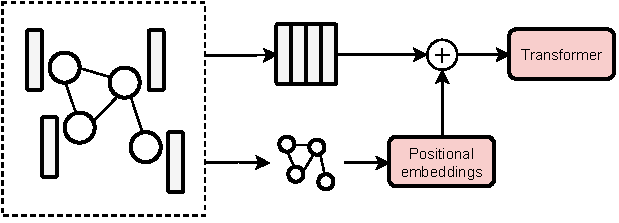
\includegraphics[width=0.6\textwidth]{images/graph_transformer}
    \caption{General idea of a graph transformer: the connectivity is embedded into a set of positional embeddings, which are added to the collected features. The result is then processed by a standard transformer network.}
    \label{fig:graph_transformer}
\end{SCfigure}

Each row of $\text{Embedding}(\mathbf{A})$ provides a vectorial embedding of the connectivity of the graph relative to a single node, ignoring all features (see Figure \ref{fig:graph_transformer}). Luckily, embedding the structure of a graph into a vector space is a broad field. As an example, we describe here a common embedding procedure based on random walks \cite{dwivedi2021graph}. Recall that the following matrix:
%
$$
\mathbf{R} =\mathbf{A}\mathbf{D}^{-1}
$$
%
can be interpreted as a “random walk”, in which $R_{ij}$ is the probability of moving from node $i$ to node $j$. We can iterate the random walk multiple times, for a fixed $k$ set a priori by the user:
%
$$
\mathbf{R}, \mathbf{R}^2, \ldots,\mathbf{R}^k
$$
%
Random walk embeddings are built by collecting all the walk probabilities of a node returning on itself, and projecting them to a fixed-dimensional embedding:
%
$$
\text{Embedding}(\mathbf{A})=\begin{bmatrix} \text{diag}(\mathbf{R}) \\ \text{diag}(\mathbf{R}^2) \\ \vdots \\ \text{diag}(\mathbf{R}^k)\end{bmatrix}\mathbf{W}
$$
%
Under specific conditions on the graph structure, this can be shown to provide a unique representation for each node \cite{dwivedi2021graph}. Alternative types of embeddings can be obtained by considering eigen-decompositions of the Laplacian matrix \cite{lim2022sign}. For a fuller exposition of graph transformers, we refer to \cite{muller2023attending}. Building graph transformers opens up the possibility of GPT-like foundation models for the graph domain, and also of adding graph-based data as an additional modality to existing language models \cite{maoposition}.

\section*{From theory to practice}

\begin{wrapfigure}{r}{3.0cm}
\vspace{-5em}
\includegraphics[width=3.0cm]{images/shutterstock_2075221579.jpg}
\vspace{-2em}
\end{wrapfigure}

Handling efficiently graph data requires extensions of the basic frameworks, due to the problems described in this chapter (e.g., sparsity). Common libraries include PyTorch Geometric for PyTorch, and Jraph for JAX. Both have ample sets of tutorials, for example for node classification in small citation networks.\footnote{Recommended example in PyTorch Geometric: \url{https://pytorch-geometric.readthedocs.io/en/latest/get_started/introduction.html}.}

\begin{SCfigure}
    \centering
    \hspace{1em}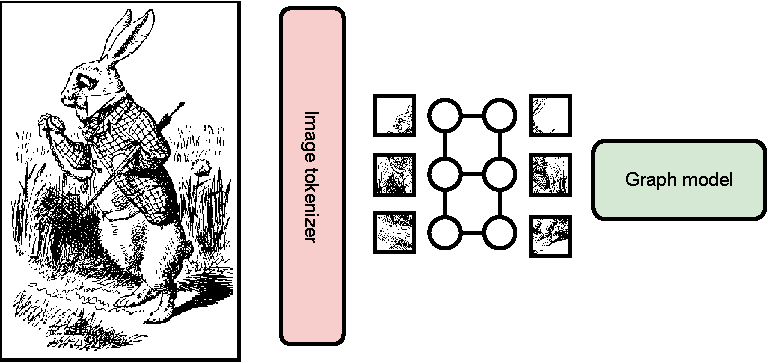
\includegraphics[width=0.6\textwidth]{images/ImageGNN}
    \caption{A GNN for computer vision: the image is tokenized into patches, an adjacency matrix is built over the patches, and the two are propagated through a graph model.}
    \label{fig:image_gnn}
\end{SCfigure}

If you implemented a Vision Transformer in Chapter \ref{chap:transformers_in_practice}, I suggest a funny exercise which has (mostly) didactic value, as shown in Figure \ref{fig:image_gnn}. Suppose we tokenize the image into patches, but instead of adding positional embeddings, we construct an adjacency matrix $\mathbf{A} \sim (p, p)$ (where $p$ is the number of patches) as:
%
\begin{equation}
A_{ij} = \begin{cases} 1 & \text{ if the two patches share a border in the image} \\ 0 & \text{ otherwise} \end{cases}
\label{eq:image_adjacency_matrix}
\end{equation}

We now have a graph classification dataset, where the node features are given by the patch embedding, and the adjacency matrix by \eqref{eq:image_adjacency_matrix}. Thus, we can perform image classification by adapting the GNN from the previously-mentioned tutorials.